\documentclass[12pt]{article}
\usepackage[english]{babel}
\usepackage{natbib}
\usepackage{url}
\usepackage[utf8x]{inputenc}
\usepackage{amsmath}
\usepackage{graphicx}
\graphicspath{{images/}}
\usepackage{parskip}
\usepackage{fancyhdr}
\usepackage{vmargin}
\usepackage{xcolor}
\usepackage{siunitx}
\usepackage{physics}
\setmarginsrb{3 cm}{2 cm}{3 cm}{2 cm}{1 cm}{1.5 cm}{1 cm}{1.5 cm}

\title{Lab 05}													% Title
\author{G 03}														% Author
\date{16 apr 2019}														% Date

\makeatletter
\let\thetitle\@title
\let\theauthor\@author
\let\thedate\@date
\makeatother

\pagestyle{fancy}
\fancyhf{}
\rhead{\theauthor}
\lhead{\thetitle}
\cfoot{\thepage}
\newcommand{\mis}[3]{(#1 \pm #2) \ #3}
\newcommand{\misp}[3]{(#1 \#3 \pm #2}
\begin{document}

%%%%%%%%%%%%%%%%%%%%%%%%%%%%%%%%%%%%%%%%%%%%%%%%%%%%%%%%%%%%%%%%%%%%%%%%%%%%%%%%%%%%%%%%%

\begin{titlepage}
	\centering
    \vspace*{0.5 cm}
    
\includegraphics[scale = 0.75]{polito.jpg}\\[1.0 cm]				% University Logo
    \textsc{\LARGE Politecnico di Torino}\\[2.0 cm]						% University Name
	\textsc{\Large Digital systems electronics\\ A.A. 2018/2019}\\[0.5 cm]		% Course Code
	\textsc{\Large Prof. G. Masera}\\[0.5 cm]		% Nome del Professore
	\rule{\linewidth}{0.2 mm} \\[0.4 cm]
	{ \huge \bfseries \thetitle \\ \small \thedate}\\
	\rule{\linewidth}{0.2 mm} \\[1.5 cm]
	
	\begin{minipage}{0.4\textwidth}
		\begin{flushleft} \large
			Berchialla Luca\\												%Cognomi e nomi
			Laurasi Gjergji
			\\
			
			Mattei Andrea\\
            Lombardo Domenico Maria\\
            
			\end{flushleft}
			\end{minipage}~
			\begin{minipage}{0.4\textwidth}
            
			\begin{flushright} \large
			236032\\													%Matricole
			238259\\
            233755\\
            233959\\
            
		\end{flushright}
        
	\end{minipage}\\[2 cm]
	
\end{titlepage}

%%%%%%%%%%%%%%%%%%%%%%%%%%%%%%%%%%%%%%%%%%%%%%%%%%%%%%%%%%%%%%%%%%%%%%%%%%%%%%%%%%%%%%%%%
\newpage

\section{One-Hot Finite state machine}
The FSM from the STG diagram given in $figure$ $1$ was implemented using a One-Hot state assigement shown in $figure$ $2$ with the circuit shown in $figure$ $3$. 
\begin{figure}[h]
	\centering
	\includegraphics[scale = 0.47]{immagini/Berchialla/STG.jpg}
	\caption{State diagram of the FSM}
\end{figure}
\begin{figure}[h]
	\centering
	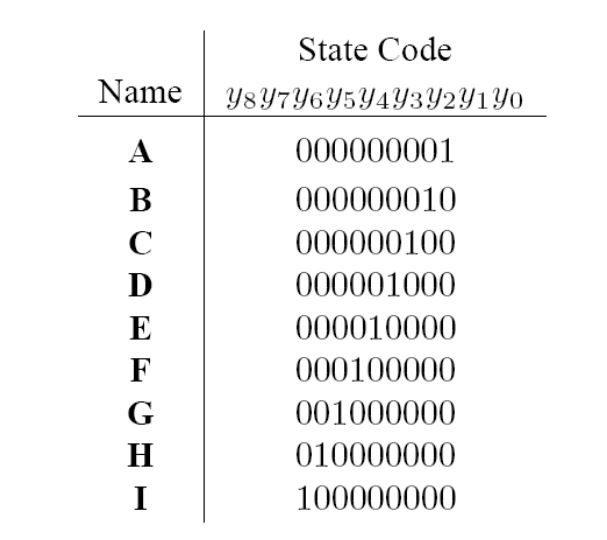
\includegraphics[scale = 0.7]{immagini/Berchialla/Code1.jpg}
	\caption{One-Hot code}
\end{figure}
\begin{figure}[h]
	\centering
	
\includegraphics[scale = 0.55]{immagini/Berchialla/RT1.jpg}
	\caption{RTL View}
\end{figure}


The correct behavior of the circuit has been verified by means of a testbench. The result of the simulation are shown in $figure$ $4$.
\begin{figure}[h]
	\centering
	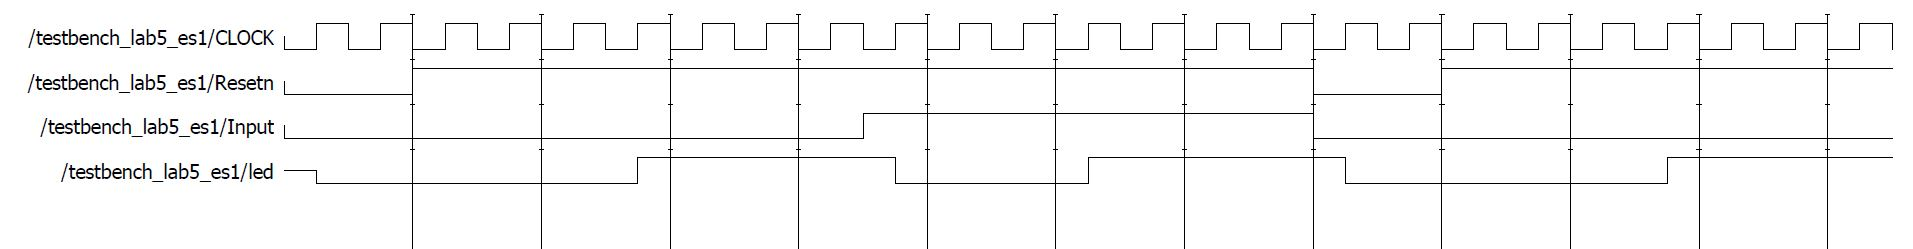
\includegraphics[scale = 0.65]{immagini/Berchialla/TB1.jpg}
	\caption{Testbench waveforms}
\end{figure}
\\
\newpage
\section{Modified One-Hot FSM}
In this section we had to implement the same FSM of the previous section, but with another One-Hot code shown in $figure$ $5$. The value of this state encoding is that the reset state is coded as $000000000$. This excludes the need of a set port for the Flip Flops in the circuit that now have only a reset port.\\
The Circuit that implements this FSM with this state encoding is shown in $figure$ $6$ and is very similar to the one of the previous section. An inverter at the output of the $y0$ Flip Flop was added while all the other connections are unchanged.
\begin{figure}[h]
	\centering
	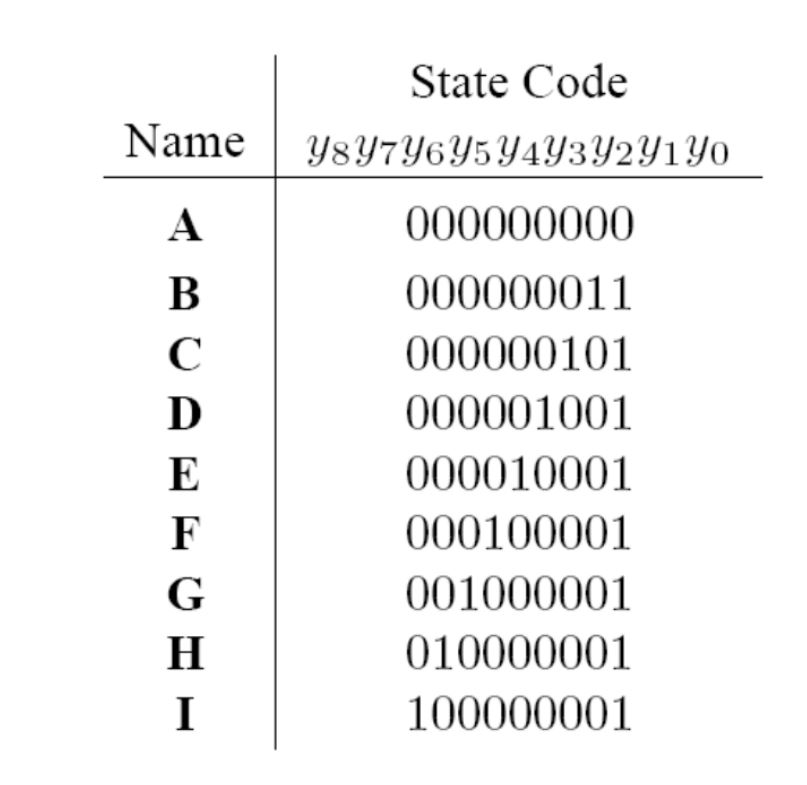
\includegraphics[scale = 0.7]{immagini/Berchialla/Code2.jpg}
	\caption{Modified One-Hot code}
\end{figure}
\section{Two-process FSM}
The task of this part is to provide an alternative implementation of the previous FSM. This implementation is composed of 3 processes each describing one of the 3 fundamental components of a generic FSM (2 combinational and 1 sequential): the first combinational circuit determines the future state based on the current state and inputs, the other combinational circuit manages the output according to the current state and the state flip-flops that store the current state. \newline
A single VHDL source file contains all the circuit. The inputs of the circuit are the first 2 switches (SW0 for the synchronous reset and SW1 for real input) and the button KEY0 used for simulating, while the sole single bit output drives the LEDR0 LED.
Using this architecture, Quartus Prime during compilation successfully recognizes that the circuit is a state machine and generates the relative state diagram, which corresponds to the desired one. \newline
The circuit was tested using a testbench that generates all the possible state transitions. The same testbench tested also the synchronous reset mechanism.
\begin{figure}[h]
	\centering
	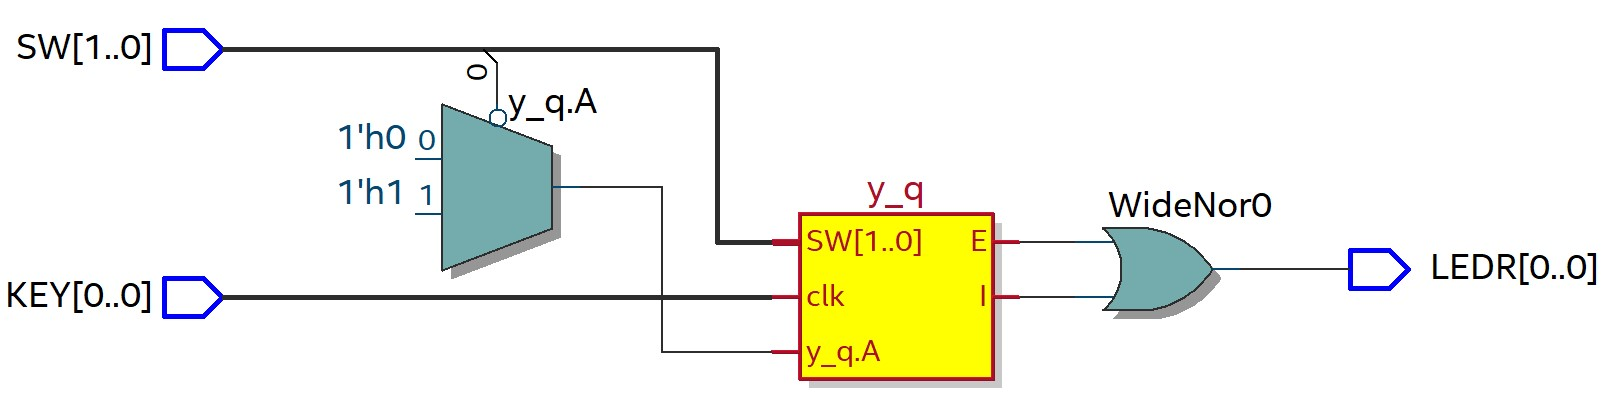
\includegraphics[scale = 0.45]{immagini/AndreaMattei/RTL5_3.jpg}
	\caption{The RTL generated of the state machine of part 3}
\end{figure}
\begin{figure}[h]
	\centering
	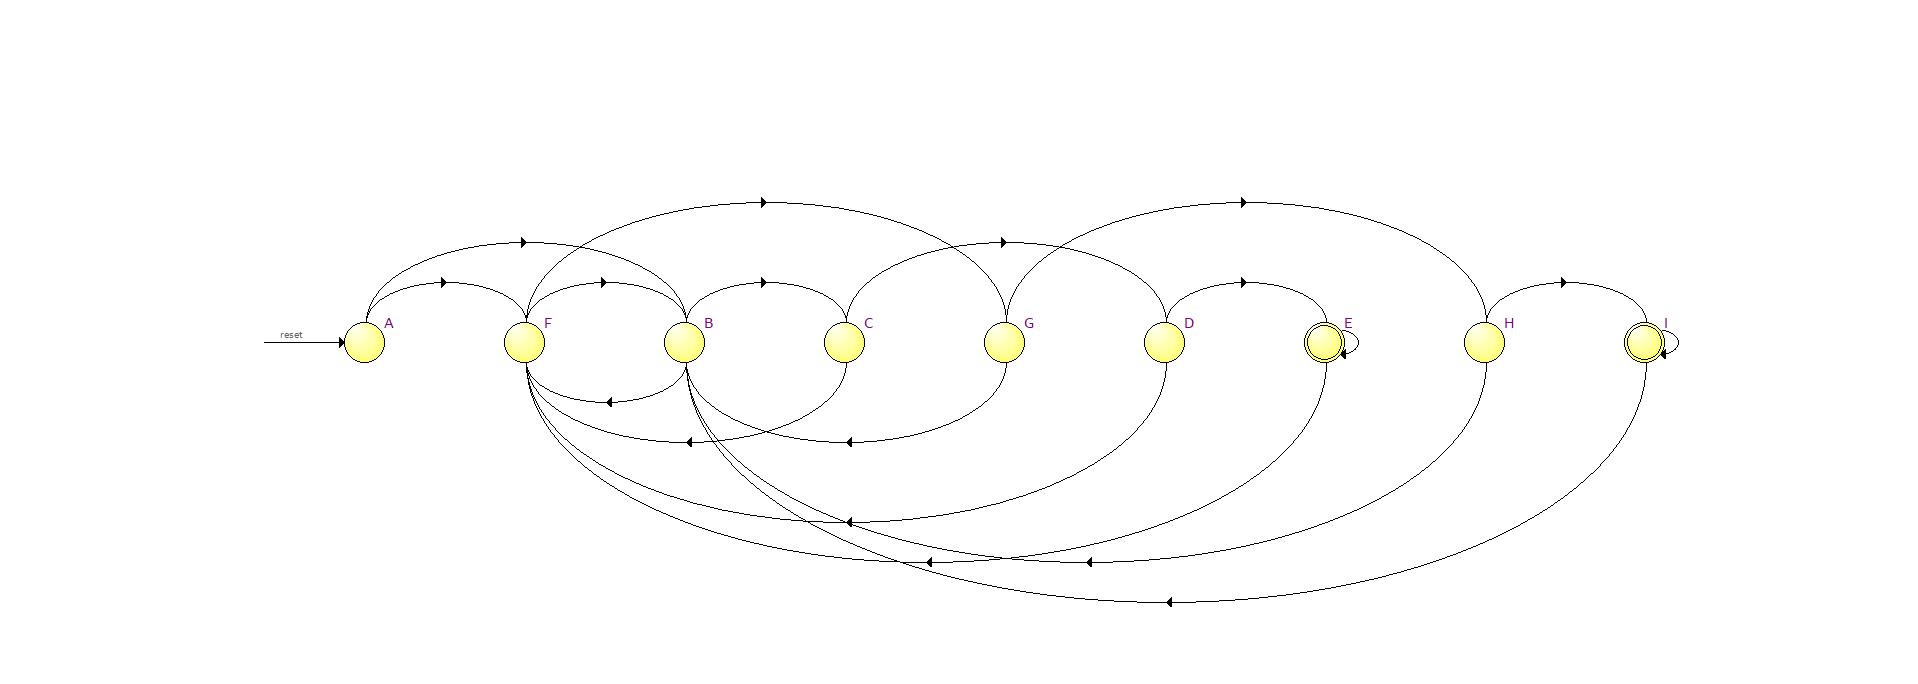
\includegraphics[scale = 0.4]{immagini/AndreaMattei/state_machine_5_3.jpg}
	\caption{The state diagram of the state machine of part 3}
\end{figure}
\newpage
\section{- “HELLO” FSM}
In this section a circuit that scrolls the word "HELLO" over the display has been implemented.
The image below shows the architecture of the circuit generated using a VHDL description:

\begin{figure}[h]
	\centering
	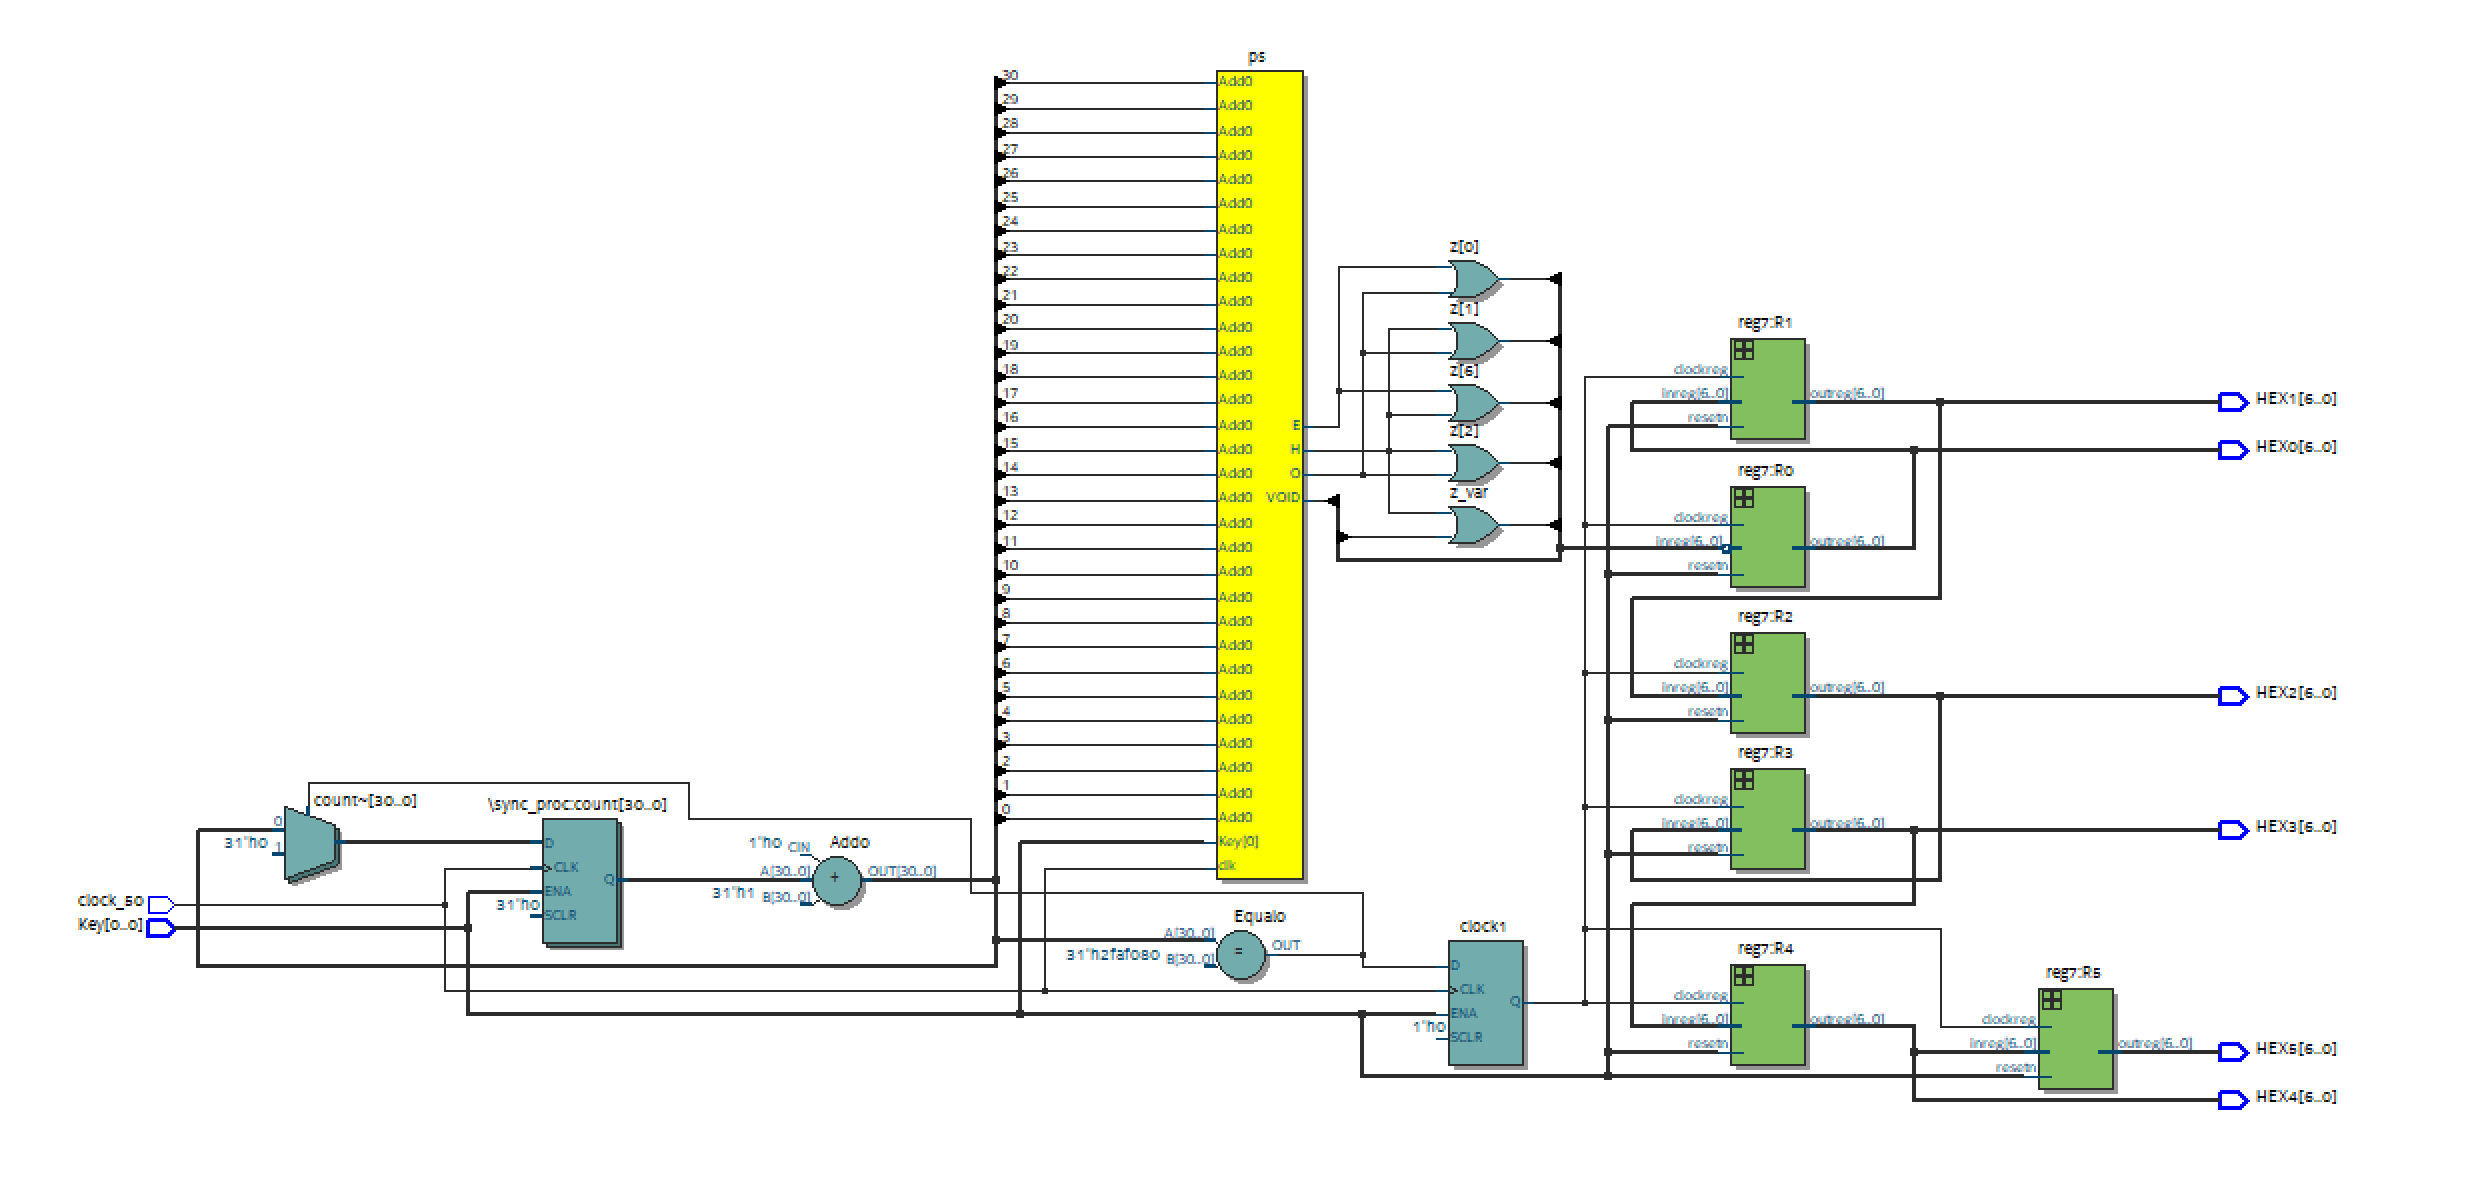
\includegraphics[scale = 0.47]{immagini/niki/rtl.PNG}
	\caption{Implemented architecture}
\end{figure}

The circuit uses six 7-bit registers connected in a pipeline fashion. Each of them directly drives a 7-segment display. 

The FSM controls the pipeline by inserting the characters (H,E,L,L,O) into the first 7-bit register.
Every second the letters scroll  from right to left, once the cycle is completed (i.e. The 'O' letter reach the leftmost display) the FSM starts the process again in an infinite loop.
The state diagram of the implemented FSM is shown below:
\begin{figure}[!h]
	\centering
	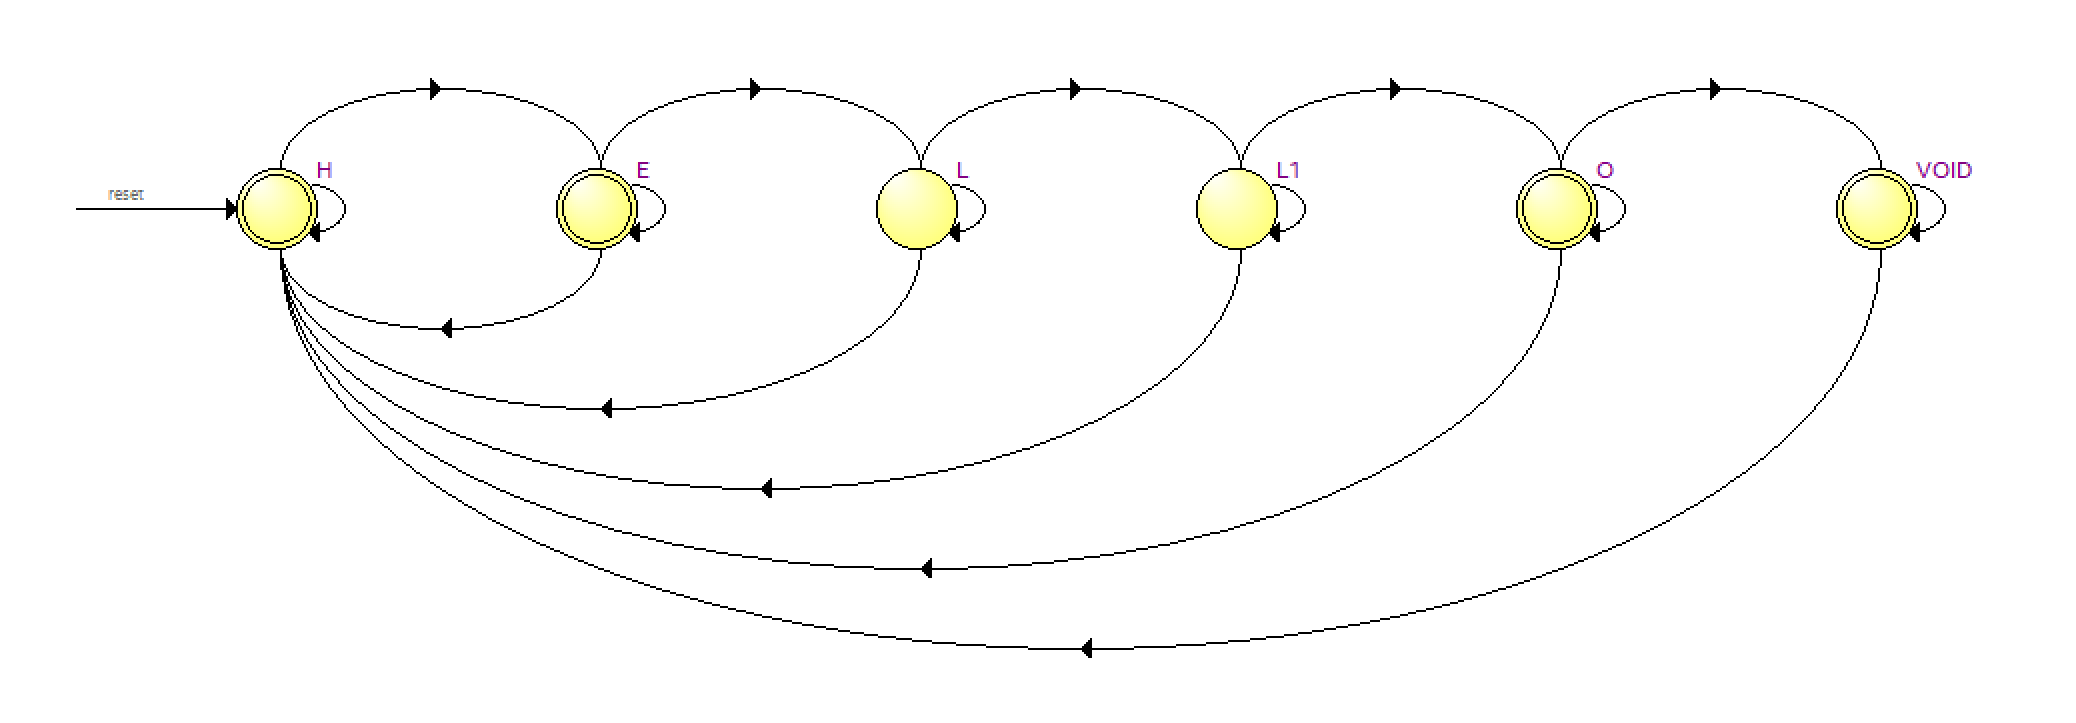
\includegraphics[scale = 0.45]{immagini/niki/statemachine.PNG}
	\caption{State Diagram}
\end{figure}
\newpage
The 6 7-bit resisters have been implemented using a behavioral approach. The testbench shown below has been performed to check their functionalities:
\begin{figure}[!h]
	\centering
	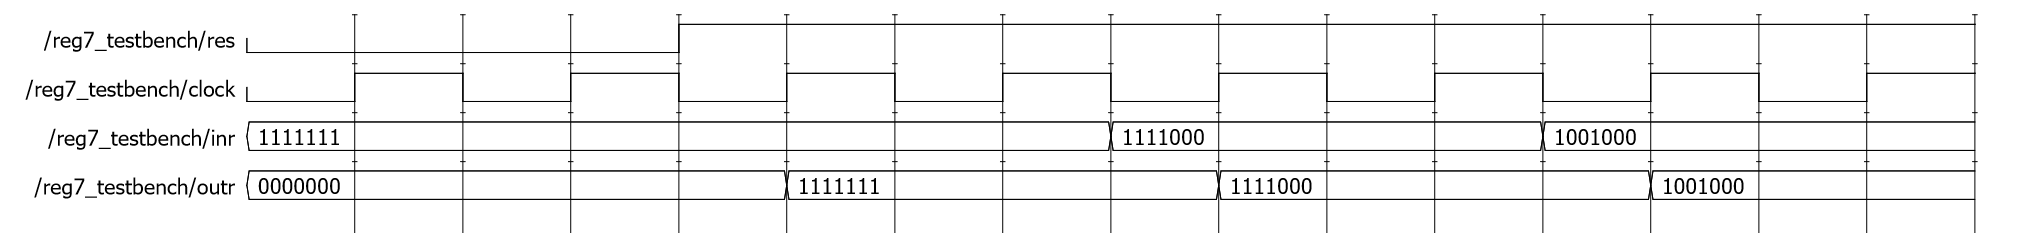
\includegraphics[scale = 0.55]{immagini/niki/reg.PNG}
	\caption{7-bit register testbench}
\end{figure}

Finally a testbench for the entire design has also been implemented, showing the correct behavior of the circuit.
\begin{figure}[!h]
	\centering
	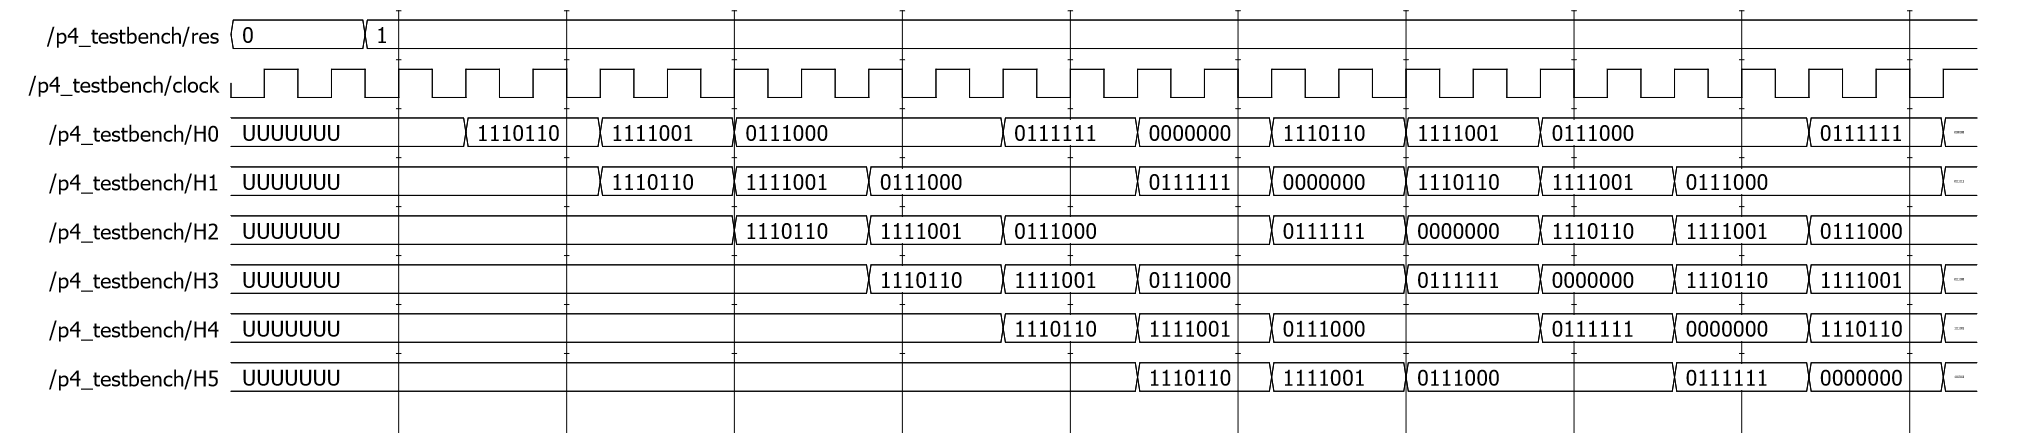
\includegraphics[scale = 0.55]{immagini/niki/disp.PNG}
	\caption{"HELLO" FSM testbench}
\end{figure}

Note that to keep the simulation fast enough the letter scrolls every 2 clock cycles.









\end{document}
